\chapter{Implementaci\'{o}}
\label{cha:implementation}
En aquest capítol es descriuen les tecnologies estudiades, escollides i aplicades per implementar el disseny anteriorment descrit.

\section{Estudi previ de les tecnologies}
En aquesta secci\'{o} es far\'{a} una descripci\'{o} de les tecnologies estudiades per la realització d'aquest projecte. S'han avaluat diferents marcs de treballs(\textit{framework}) així com un propi per la implementació del projecte.\\

A continuació fem una anàlisis de cadascuna de elles explicant els avantatges i desavantatges.

\subsection{Llenguatge de programació: JAVA vs. PHP}
S'han avaluat dos llenguatges de programació: JAVA i PHP.\\

En un principi es va avaluar JAVA per el desenvolupament dels servei web amb un \texit{framework} anomenat \textit{Jersey}.\cite{jersey} Aquesta tecnologia implementa llibreries API de tipus RESTful, molt convenient per entorns distribuits, però t\'{e} l'impediment de tenir d'una corba de desenvolupament molt lenta i un integració entre components externs complexes. Això era un impediment ja que la integració amb el sistema de cues \'{e}s un requeriment. L'altre gran desavantatge era que implicava un canvi de disseny en la capa de presentació. S'hauria d'aplicar el patró MVC(explicat a la secció \ref{mvcFrontController}) als navegadors amb tecnologies mitjançant l'us de \textit{frameworks} que encara estan en etapes de desenvolupament i/o evolució.\\

PHP \'{e}s l'altre llenguatge analitzat. PHP \'{e}s un llenguatge orientat objectes enfocat al desenvolupament web que:
\begin{itemize}
\item \'{e}s àmpliament usat.
\item \'{e}s àmpliament reconegut.
\item t\'{e} una documentació excel·lent.
\item t\'{e} una comunitat activa i participativa.
\item les ultimes versions desenvolupades han tingut molt bons resultats en rendiments i en escal.labilitat.
\item \'{e}s de desenvolupament ràpid.
\end{itemize}

\subsection{Motor de base de dades}
S'han evaluat i testat dos motors de bases de dades: MySQL i MongoDB.\\

MongoDB \'{e}s un motor de base de dades orientat a documents molt escal·lable i d'alt rendiment. \'{E}s un tipus de base de dades "NOSql"; es a dir no relacional. MongoDB gestiona col·leccions de documents en format JSON.\cite{apijson} Una gran avantatge d'aquest motor \'{e}s la llibertat de no definir cap estructura predeterminada pels documents. Una avantatge molt interessant per la gestió de dades de matrius.\cite{mongodb}\\

Però el gran problema que trobem en MongoDB per aquest projecte \'{e}s la absència del model relacional. \'{E}s molt important el requeriment relacional de dades per gestionar la associació entre conjunts de fitxers, els fitxers i les variables. MongoDB \'{e}s un motor de base de dades no relacional. Per establir relacions s'han de forçar les relacions amb el cost de implementar-les en el codi i amb estructures extraordinàries dintre del motor de base de dades.\\

Els requeriments dels projecte recomanen l'us d'una base de dades relacional. MySQL, pel contrari de MongoDB, \'{e}s un motor de base de dades relacionals àmpliament usat en el desenvolupament web. Implementant el disseny del model de bases dades(mirar la seccio \ref{subsec:diagramclasses}) vam veure que tenia un rendiment excel·lent en la creació de matrius i en la gestió de configuracions de matrius.

\subsection{Anàlisis de marcs de treball}
Una vegada seleccionats el llenguatge de programació i el motor de bases de dades, s'han analitzat diferents marcs de treball per la implementació del projecte. A continuació analitzem les avantatges i desavantatges de cadascun.

\subsubsection{\textit{Framework} a mida}
En un principi \'{e}s va valorar la possibilitat de desenvolupar tot un nou \textit{framework} per la implementaci\'{o} del projecte.\\

Els principal avantatges \'{e}s el control total de la implantaci\'{o} de tots els processos i tecnologies.\\

Els principals inconvenients son:
\begin{itemize} 
\item desenvolupament extremadament lent.
\item re-inventar la roda quan no \'{e}s necessari. Existeixen al mercat marcs de treballs excel·lents i que compleixen les necessitats requerides.
\end{itemize} 

\subsubsection{\textit{Codeigniter}}
Es va avaluar el desenvolupar del sistema amb \textit{Codeigniter}. \textit{Codeigniter} \'{e}s un \textit{framework} per a desenvolupament web r\`{a}pid amb PHP.\cite{codeigniter} Implementa el patro MVC(mirar la secció \ref{subsec:dessignexplanation}) amb un patró de persistència de dades de tipus ''active record' per la gesti\'{o} d'emmagatzematge de dades.\cite{activerecord}\\

Els principals avantatges son:
\begin{itemize}
\item corba d'aprenentatge r\`{a}pida.
\item desenvolupament r\`{a}pid.
\item implementa el patr\'{o} MVC(mirar la secció \ref{subsec:dessignexplanation}).
\end{itemize}

Els principals inconvenients son:
\begin{itemize}
\item no compleix tots el requisits de disseny de patrons especificat.
\item no inclou \textit{templating}
\item dificultat en segregar la l\`{o}gica de la presentaci\'{o}.
\end{itemize}

Els desavantatges de no complir cap dels dissenys especificats, a excepció del patró MVC, han sigut decisius per no usar aquesta tecnologia.

\subsubsection{\textit{Symfony2}}
Finalment es va estudiar les tendències actuals i es va decidir estudiar \textit{Symfony2}.\cite{symfony} \textit{Symfony2} \'{e}s un HTTP \textit{framework} per a PHP. Nativament implementa una variaci\'{o} del Model-Vista-Controlador amb controlador frontal amb injecci\'{o} de depencies a la capa de serveis(mirar la secció \ref{subsec:dessignexplanation}).\\

Els principals avantatges son:
\begin{itemize}
\item Altament configurable.
\item Compleix tots els requisits de dissenys de patrons especificat.
\item Alt rendiment
\end{itemize}

Els principal inconvenients \'{e}s que t\'{e} una corba d'aprenentatge alta.\\

Els avantatges han fet que es decidís per usar aquesta tecnologia. \textit{Symfony2} utilitza un conjunt de tecnologies que fan que s'implementi correctament la especificació i s'assoleixi tots els requeriments especificats. A continuació es descriu breument el \textit{framework} i totes les tecnologies involucrades.

\section{Implementaci\'{o}}
El sistema ha sigut desenvolupat principalment amb el \textit{framework} \textit{Symfony2}. A continuaci\'{o} es dona una visi\'{o} general del \textit{framework} i a la implementació del projecte.

\subsection{\textit{Symfony2}}
Arquitectonicament, \textit{Symfony2} estructura el codi en \textit{Bundles}, similar als paquets de JAVA. Els \textit{bundles} son un conjunt de serveis, entitats i recursos independents entre si. Els \textit{bundles} implementats son:
\begin{itemize}
\item \textit{Bundle} de usuaris: UserBundle. Paquet de serveis, vistes i recursos per usuaris. S'ha utilitzat el paquet de \textit{Symfony2} FOSUserBundle \cite{fosuserbundle} i s'ha fet una extensi\'{o} del paquet per implementar la gesti\'{o} de rols i grups. 
\item \textit{Bundle} de matrius: MatrixBundle. Paquet de serveis, vistes i recursos per les matrius.
\item \textit{Bundle} de trainings: TrainingBundle. Paquet de serveis, vistes i recursos per els entrenaments.
\item \textit{Bundle} de serveis webs: ApiBundle. Paquet de serveis,vistes i recursos per la API JSON Restful. 
\item \textit{Bundle} de predicci\'{o}: PredictionBundle. Paquet de serveis, vistes i recursos per les matrius de prediccions.
\end{itemize}

\subsection{Gesti\'{o} de depend\`{e}ncies} 
\textit{Symfony2} utilitza \textit{Composer} per la gesti\'{o} de depend\`{e}ncies.\cite{composer} \textit{Composer} \'{e}s un gestor de dependencies a nivell d'aplicaci\'{o}. Les depend\`{e}ncies son:
\begin{itemize}
\item Jquery: llibreria Javascript que s'executa en el costat client per enriquir les interfícies. Simplifica la manera de interaccionar amb els documents HTML i la simplifica la manera de manipular l'arbre DOM.\cite{jquery}
\item FOSUserBundle: paquet per a \textit{Symfony} per la gesti\'{o} de usuaris.\cite{fosuserbundle}
\item Bootstrap: \texit{framework} pel \textit{front-end} desenvolupat per Twitter. Implementa nous estàndards com HTML5 i CSS3. Permet el desenvolupament d'interf\'{i}cies de manera r\`{a}pida i usables suportades per múltiples navegadors.
\item RestBundle: paquet per Symfony per desenvolupar llibreries API JSON Restful.\cite{apijson}
\item Symfony FS: paquet per gestionar sistema de fitxers.
\item Doctrine Fixtures: paquet per gestionar la inserci\'{o} controlada de dades a la base de dades.
\item TWIG: motor de plantilles per a PHP.\cite{twig}
\item Doctrine: ORM pel mapatge de dades, usant MySQL.\cite{mysql}
\item Sistema de cues: projecte desenvolupat per Miguel Ibero conjuntament amb aquest per la execució de Ichnaea.
\end{itemize}

\subsection{Recursos}
L'estandard HTTP recomana unes URI estructurades i coherents.\cite{rfc3986} La dependència de les nostres entitats requereixen una definició jeràrquica del recursos webs. La estructura de recursos de la aplicaci\'{o} \'{e}s la següent:\\

\begin{table}
\begin{tabular}{| p{5cm} | p{10cm} |}
\hline
Matrius     & matrix/(id) \\ \hline
Entrenamens & matrix/(id)/training/(id) \\ \hline
Prediccions & matrix/(id)/training/(id)/prediction/(id) \\ \hline
Fitxers 	& season/(id) \\ \hline
Variables	& variable/(id) \\ \hline
Conjunt de fitxers d'una variable & variable/(id)/seasonset/(id) \\ \hline
Fitxer d'un conjunt de fitxers d'una variable & variable/(id)/seasonset/(id)/season/(id) \\ \hline
\end{tabular}
\caption{Taula dels recursos web de l'aplicació}
\end{table}
\\

S'ha emprat aquesta estructura de recursos degut a les dependències entre les diferents entitats. Un entrenament dep\'{e}n d'una matriu i una predicci\'{o} dep\'{e}n d'un entrenament.

\section{API: llibreria de serveis web}
S'ha desenvolupat una llibreria API JSON RESTful per donar resposta a les funcionalitats asíncrones de les interfícies.\cite{apijson} S'ha emprat aquesta tecnologia per la escal.labilitat que aporta i perquè en un futur es pugui aprofitar el desenvolupament d'aquesta amb la integració d'altres tipus client, com poden ser aplicacions mòbils o altres serveis.\\

La arquitectura RESTful aprofita al màxim el protocol HTTP per establir dades i actualment s'usen per donar funcionalitats asincrones a les interficies(mirar \ref{sec:dessigninterfaces}).

Les operacions, els recursos i el paràmetres implementats son:\\
\begin{figure}[H]
  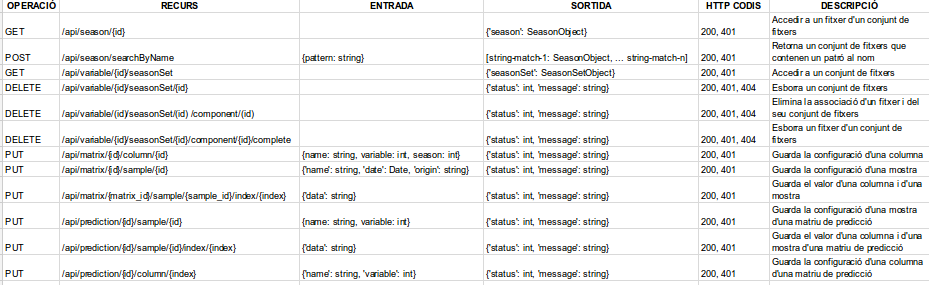
\includegraphics[scale=0.5]{img/implementation/apirestul.png}
  \caption{Operacions de la API Restful}
  \label{fig:apirestful}
\end{figure}
On:
\begin{itemize}
\item Operació \'{e}s el mètode HTTP.
\item Recurs \'{e}s el identificador del recurs.
\item Entrada \'{e}s l'objecte JSON d'entrada de la operació.
\item Sortida \'{e}s l'objecte JSON de sortida de la operació.
\item HTTP Codi son els codis HTTP que retornen.\cite{listhttpcodis}
\end{itemize}

Totes les operacions estan securitzades per \textit{cookies}\cite{cookies} i per sessió per identificar i validar a l'usuari.\cite{sessions}

\section{Integraci\'{o} amb el sistema de cues RabbitMQP}
\subsection{Introducci\'{o} a l'arquitectura de cues: AMQP}
\label{sec:queue_system_overview}
L'est\`{a}ndard AMQP (''Advanced Message Queuing Protocol'') \'{e}s un protocol d'est\`{a}ndard obert en la capa d'aplicacions d'un sistema de comunicació. Les característiques que defineixen al protocol AMQP son la orientació a missatges, encuament(''queuing''), enrutament i exactitud, entre altres com,per exemple, la seguretat o les subscripcions.\cite{amqp}\\

AMQP defineix una s\`{e}rie d'entitats. Des de la perspectiva de la interconnexió les m\'{e}s rellevants son:
\begin{itemize}
\item El corredor de missatges: un servidor on els clients AMQP es connecten usant el protocol AMQP. Els corredores de missatges poden executar-se en un entorn distribuït, però aquesta capacitat \'{e}s espec\'{i}fica de la implementació.
\item Usuari: un usuari \'{e}s una entitat amb credencial pot ser autoritzat a connectar-se a un corredor.
\item Connexió: una connexi\'{o} f\'{i}sica, usant per exemple TCP/IP, entre el corredor i l'usuari.
\item Clients: productors i consumidors. \'{E}s un model de comunicacio con el productor \'{e}s un proces emissor  i el consumidor \'{e}s un proces receptor.\cite{messaging}
\end{itemize}

\textbf{RabbitMQ} \'{e}s un \textit{software} que implementa aquest protocol. El sistema de cues est\'{a} implementat com a Projecte de Final de Carrera de Miguel Ibero i ofereix una llibreria per la seva integració.\\

Per la integració amb el sistema amb cues s'ha desenvolupat:
\begin{itemize}
\item Gestionar la dependència.
\item Desenvolupar el consumidors.
\end{itemize}

\subsection{Consumidors i gesti\'{o} de resultats}
Els consumidors en el protocol de missatgeria son els processos receptors de missatges emesos per els productors. Les respostes de les execucions de Ichnaea  (mirar la figura \ref{dessign:archsoftware}) les rep el consumidor. \\

\textit{Symfony2} permet crear comandes CLI per crear processos. Els consumidors necessiten ser processos ''stand-alone''(aut\'{o}noms) que escoltin les sortides i consumeixin els resultats de la cua. \\

L'esquelet d'una comanda per aquests consumidors actualment \'{e}s:
\begin{lstlisting}
class ConsumerCommand extends ContainerAwareCommand
{
	//Definicio de la comanda
	protected function configure()
	{
		$this
		->setName('nom_de_la_comanda')
		->setDescription('Consumer server');
	}
	
	//Execucio de la comanda
	protected function execute(InputInterface $input, OutputInterface $output)
	{
		//Interficie per integrar el sistema de cues
		$amqp = new AmqpConnection('URI_per_fer_la_connexio');
		$amqp->open();
		
		//Crida al servei
		$servei = $this->getContainer()->get('nom_de_servei');
		
		//Crear el consumidor, amb una 
		//funcio que es crida quan la 
		//cua estableix comunicacio amb 
		//un objecte de la resposta esperada 
		//i li passa el servei 
		$amqp->listenForBuildModelResponse(function (ObjectResponse $resposta_de_la_cua) use ($servei){
		 	//Codi servidor
		 	....
			$servei->actualitzaDades($resposta_de_la_cua);
			....
		});
		$amqp->wait();
	}
}
$end
\end{lstlisting}

\subsubsection{Consumidor d'entrenaments}
El consumidor d'entrenaments escolta les respostes del productor d'entrenaments. \\

Ichnaea actualment no retorna progres parcial ni estimacions de finalitzaci\'{o}. Solament produeix un resultat al final de la seva execució. Es a dir, en el tros de codi servidor simplement escoltar totes les sortides i enviar-les al servei d'entrenaments.

\begin{lstlisting}
$trainingService = $this->getContainer()->get('ichnaea.training_service');
		
$amqp->listenForBuildModelResponse(function (BuildModelsResponse $resp) use ($trainingService){
	$data = $resp->toArray();
	var_dump($data);
	$trainingService->updateTraining($resp->getId(), $data['progress'], $data['error'], $data['data'] );
});
$amqp->wait();
\end{lstlisting}

Els missatges produïts son vectors associatius que conte el identificador del proces i els binaris retornats. Aquests binaries son un fitxer en format zip en Base64 que cont\'{e} les dades per poder usar-les en les prediccions.

\subsubsection{Consumidor de prediccions}
El consumidor de prediccions escolta les respostes del productor de prediccions.\\

La execució d'Ichnaea per prediccions treu resposta per cadascuna de les mostres proporcionades. Peró no son totes valides. La resposta s'ha d'avaluar segons la especificació donada. 
\begin{lstlisting}
$predictionService = $this->getContainer()->get('ichnaea_web_app_prediction.service');
		
$amqp->listenForPredictModelsResponse(function (PredictModelsResponse $resp) use ($predictionService){
	$data = $resp->toArray();
	
	$data['result'] = $resp->getResult();

	if($resp->getResult()->isFinished()) {
 		$data['result'] = $resp->getResult();
	} else {
		unset($data['result']);
	}
	$predictionService->updatePrediction($resp->getId(), $data['progress'], $data['error'], isset($data['result']) ? $data['result'] : 'NULL');
		});
		$amqp->wait();
\end{lstlisting}

Els missatges produïts son vectors associatius que cont\'{e} el identificador del proces i resultats. Els resultats son uns objectes que es guarden contínuament en un vector de resultats.


\section{Serveis Web Ichnaea}
Un cop explicat quins són els llenguatges, les eines de desenvolupament i les tecnologies que s’han fet servir en la realització d’aquest projecte, es pot veure el sistema d’informació resultant a l'apendix \ref{cha:userguide}
i a l'apendix \ref{cha:adminguide}.\\ 
 